\section{Introduction}

With the development of quantum computing, quantum algorithms have been proposed to solve various problems more efficiently than classical algorithms. \\
One of the most famous quantum algorithms is \textbf{Shor's algorithm} for integer factorization, which can factorize large integers in polynomial time, while the best-known classical algorithms run in sub-exponential time. 
\\
Another important quantum algorithm is \textbf{Grover's algorithm} for unstructured search, which provides a quadratic speedup over classical algorithms.
\medskip

\noindent
Classic cryptographic protocols, such as RSA and ECC, rely on the hardness of certain mathematical problems, like integer factorization and discrete logarithms.\\ However, with the advent of quantum algorithms, these protocols become vulnerable to attacks performed using quantum computers. \\
This has led to the development of post-quantum cryptography, which aims to create cryptographic schemes that are secure against quantum attacks.
\medskip

\noindent
For istance, currently RSA-2048 can be broken by a quantum computer with at least \textasciitilde 4000 qubits.

\newpage
\subsection{Proposed Hard Problems}
Mathematicians have been proposed new paradigms which are based on different mathematical hard problems.

\subsubsection{Code based cryptography}

\begin{figure}[h!]
  \centering
  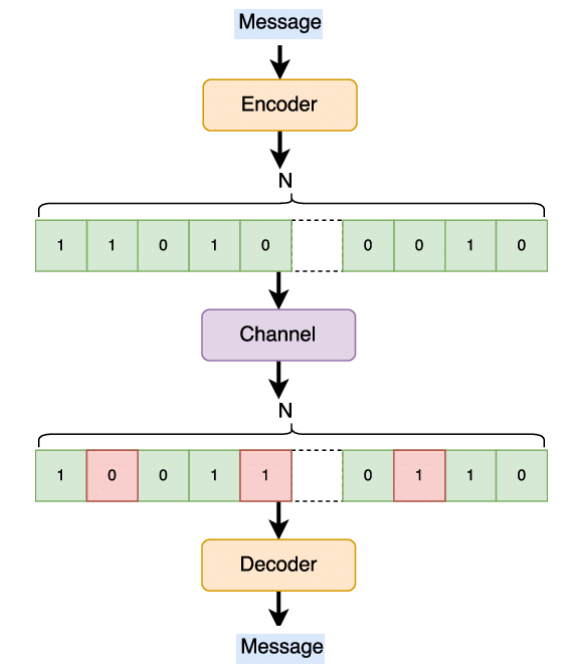
\includegraphics[width=0.5\textwidth]{images/section_1/code_base.png}
  \caption{Code-based cryptography}
  \label{fig:code-based}
\end{figure}

\noindent
Code-based cryptography is a type of post-quantum cryptography that relies on the \underline{hardness of decoding random linear codes} \\
The most well-known code-based cryptosystem is the McEliece cryptosystem, which was proposed in 1978. It is based on the difficulty of decoding a general linear code, which is believed to be resistant to quantum attacks.


\subsubsection{Lattice based cryptography}

\begin{figure}[h!]
  \centering
  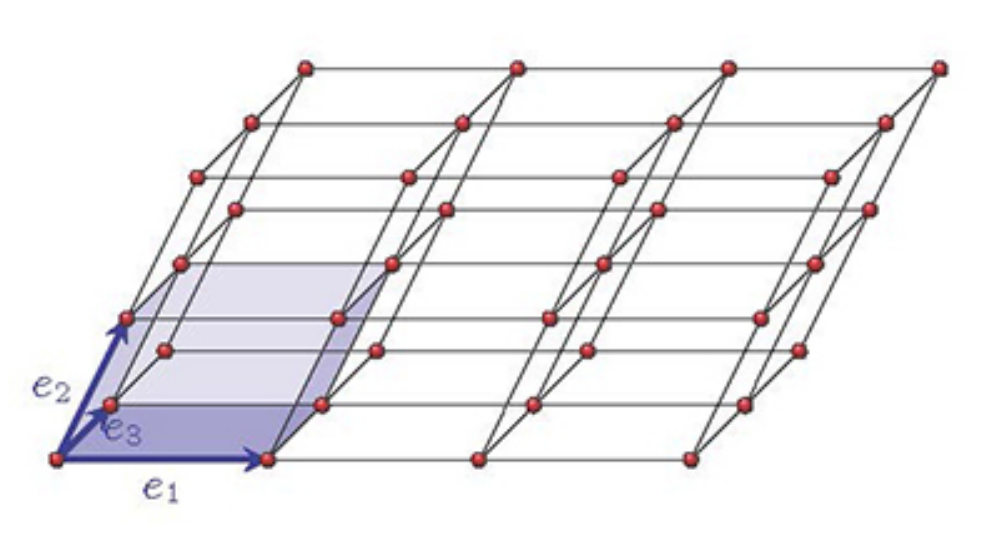
\includegraphics[width=0.75\textwidth]{images/section_1/lattice}
  \caption{Lattice based cryptography}
  \label{fig:lattice-based}
\end{figure}

Lattice based cryptography is another approach to post-quantum cryptography that relies on the hardness of certain problems in lattice theory, such as the shortest vector problem (SVP), the closest vector problem (CVP) and the learning with errors (LWE) problem. \\
These problems are believed to be resistant to quantum attacks and have gained significant attention in recent years.

\subsubsection{Multivariate cryptography}


\begin{align*}
f_1(x_1, \dots, x_n) &= \sum_{1 \leq i \leq j \leq n} a_{ij}^{(1)} x_i x_j + \sum_{1 \leq i \leq n} b_i^{(1)} x_i + c^{(1)} = 0, \\
\vspace{1cm}
f_2(x_1, \dots, x_n) &= \sum_{1 \leq i \leq j \leq n} a_{ij}^{(2)} x_i x_j + \sum_{1 \leq i \leq n} b_i^{(2)} x_i + c^{(2)} = 0, \\
\vspace{0.5cm}
&\vdots \\
\vspace{0.5cm}
f_m(x_1, \dots, x_n) &= \sum_{1 \leq i \leq j \leq n} a_{ij}^{(m)} x_i x_j + \sum_{1 \leq i \leq n} b_i^{(m)} x_i + c^{(m)} = 0.
\end{align*} 

\noindent
Multivariate cryptography is a third approach to post-quantum cryptography that relies on the hardness of solving systems of multivariate polynomial equations of degree at least two. 


\subsection{NIST standardization}
In 2017, NIST (National Institute of Standards and TechnologyUSA) opened a call for submitting new post-quntum cryptographic schemes and digital signatures, with three rounds, divided into:
\begin{itemize}
\item Key Encapsulation Mechanism (KEM)
\item Digital Signatures
\end{itemize}

\noindent
Initially, 82 proposals were submitted to the NIST PQC competition, and 69 were admitted to the first round. In July 2022, NIST announced the selected algorithms after the third round.

\paragraph{Selected Algorithms (Round 3)}

\begin{itemize}
    \item \textbf{Lattice-based}
    \begin{itemize}
        \item \textbf{KEM}: CRYSTALS-Kyber
        \item \textbf{Digital Signatures}: CRYSTALS-Dilithium, Falcon
    \end{itemize}
    
    \item \textbf{Hash-based}
    \begin{itemize}
        \item \textbf{Digital Signatures}: SPHINCS+
    \end{itemize}
\end{itemize}

\paragraph{Round 4 Candidates}

\begin{itemize}
    \item \textbf{Code-based KEM}: BIKE, Classic McEliece, HQC
    \item \textbf{Isogeny-based}: SIKE (broken in August 2022)
\end{itemize}

\paragraph{New NIST Call for Digital Signatures (2024)}

\noindent
After the first round (October 2024), 14 signature schemes remain in the competition:

\begin{itemize}
    \item \textbf{Lattice-based}: HAWK
    \item \textbf{Code-based}: CROSS, LESS
    \item \textbf{MPC-in-the-Head}: Mirath, MQOM, PERK, RYDE, SDitH
    \item \textbf{Multivariate}: MAYO, QR-UOV, SNOVA, UOV
    \item \textbf{Isogeny-based}: SQIsign
    \item \textbf{Symmetric-based}: FAEST
\end{itemize}


\newpage

\subsection{NOT-Covered Hard Problem}
The following hard problems are not covered in this course, but they are also important in the context of post-quantum cryptography:

\subsubsection{Hash based cryptography}

\begin{figure}[h!]
  \centering
  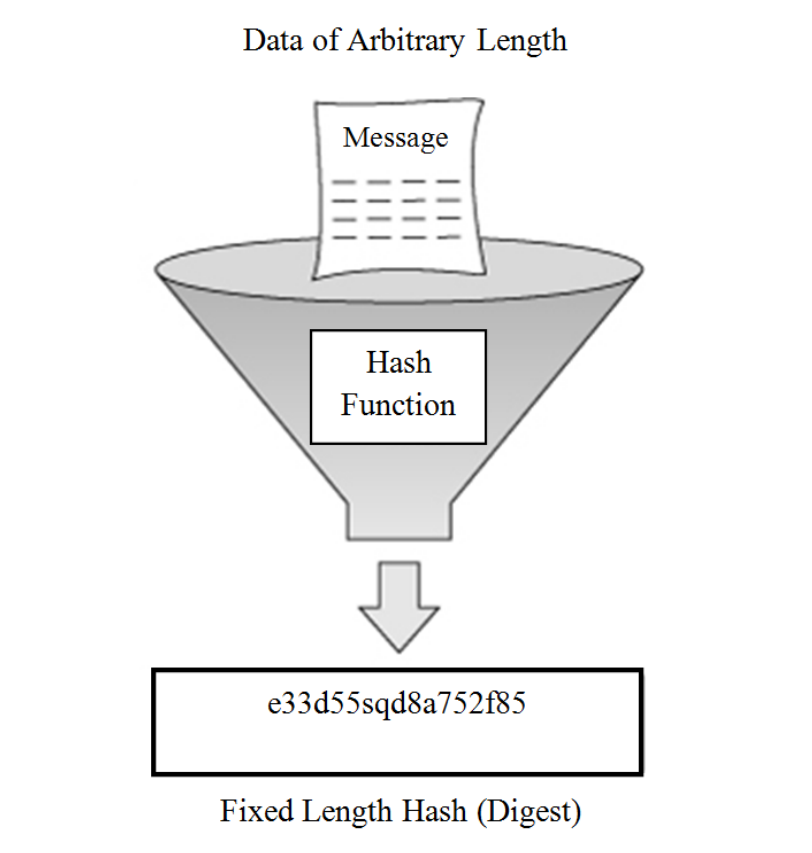
\includegraphics[width=0.5\textwidth]{images/section_1/hash_based.png}
  \caption{Hash based cryptography}
  \label{fig:hash-based}
\end{figure}

\noindent
Hash-based cryptography relies on the hardness of finding collisions in hash functions. It is a well-studied area of post-quantum cryptography, and several hash-based signature schemes have been proposed, such as the Merkle signature scheme and the SPHINCS.

\subsubsection*{Isogeny based cryptography}

\begin{figure}[h!]
  \centering
  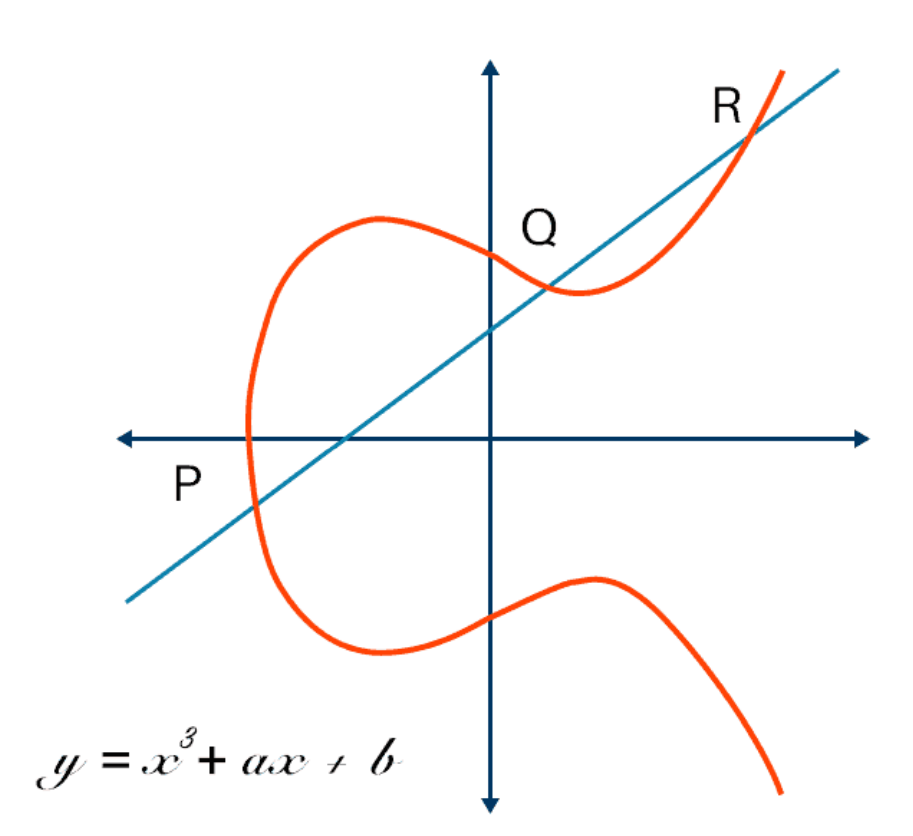
\includegraphics[width=0.5\textwidth]{images/section_1/isogeny.png}
  \caption{Isogeny based cryptography}
  \label{fig:isogeny-based}
\end{figure}

Isogeny-based cryptography relies on the hardness of finding isogenies between elliptic curves \textit{"given two elliptic curves, finding a path between them"}. It is a relatively new area of post-quantum cryptography, and several isogeny-based schemes have been proposed, such as the Supersingular Isogeny Key Exchange (SIKE) protocol [recently broken in August 2022].

\newpage

\subsection{Focus: Quantum Notation}
\[
|\psi\rangle = a|0\rangle + b|1\rangle,
\qquad a,b \in \mathbb{C}
\]

\[
|a|^2 + |b|^2 = 1
\]

\[
|0\rangle =
\begin{pmatrix}
1 \\
0
\end{pmatrix},
\qquad
|1\rangle =
\begin{pmatrix}
0 \\
1
\end{pmatrix}
\]

\[
|\psi\rangle =
a
\begin{pmatrix}
1 \\
0
\end{pmatrix}
+
b
\begin{pmatrix}
0 \\
1
\end{pmatrix}
=
\begin{pmatrix}
a \\
b
\end{pmatrix}
\in \mathbb{C}^2
\]

\[
|\psi\rangle =
\frac{1}{\sqrt{2}}|0\rangle +
\frac{1}{\sqrt{2}}|1\rangle
=
\frac{1}{\sqrt{2}}
\begin{pmatrix}
1 \\
1
\end{pmatrix}
\]

\noindent
In quantum computing, the state of a qubit is represented as a linear combination of the basis states $|0\rangle$ and $|1\rangle$, where the coefficients $a$ and $b$ are complex numbers that satisfy the normalization condition $|a|^2 + |b|^2 = 1$. The basis states can be represented as column vectors, and the state of the qubit can be expressed as a vector in a two-dimensional complex Hilbert space.


